\documentclass{article}\usepackage[]{graphicx}\usepackage[]{color}
%% maxwidth is the original width if it is less than linewidth
%% otherwise use linewidth (to make sure the graphics do not exceed the margin)
\makeatletter
\def\maxwidth{ %
  \ifdim\Gin@nat@width>\linewidth
    \linewidth
  \else
    \Gin@nat@width
  \fi
}
\makeatother

\definecolor{fgcolor}{rgb}{0.345, 0.345, 0.345}
\newcommand{\hlnum}[1]{\textcolor[rgb]{0.686,0.059,0.569}{#1}}%
\newcommand{\hlstr}[1]{\textcolor[rgb]{0.192,0.494,0.8}{#1}}%
\newcommand{\hlcom}[1]{\textcolor[rgb]{0.678,0.584,0.686}{\textit{#1}}}%
\newcommand{\hlopt}[1]{\textcolor[rgb]{0,0,0}{#1}}%
\newcommand{\hlstd}[1]{\textcolor[rgb]{0.345,0.345,0.345}{#1}}%
\newcommand{\hlkwa}[1]{\textcolor[rgb]{0.161,0.373,0.58}{\textbf{#1}}}%
\newcommand{\hlkwb}[1]{\textcolor[rgb]{0.69,0.353,0.396}{#1}}%
\newcommand{\hlkwc}[1]{\textcolor[rgb]{0.333,0.667,0.333}{#1}}%
\newcommand{\hlkwd}[1]{\textcolor[rgb]{0.737,0.353,0.396}{\textbf{#1}}}%
\let\hlipl\hlkwb

\usepackage{framed}
\makeatletter
\newenvironment{kframe}{%
 \def\at@end@of@kframe{}%
 \ifinner\ifhmode%
  \def\at@end@of@kframe{\end{minipage}}%
  \begin{minipage}{\columnwidth}%
 \fi\fi%
 \def\FrameCommand##1{\hskip\@totalleftmargin \hskip-\fboxsep
 \colorbox{shadecolor}{##1}\hskip-\fboxsep
     % There is no \\@totalrightmargin, so:
     \hskip-\linewidth \hskip-\@totalleftmargin \hskip\columnwidth}%
 \MakeFramed {\advance\hsize-\width
   \@totalleftmargin\z@ \linewidth\hsize
   \@setminipage}}%
 {\par\unskip\endMakeFramed%
 \at@end@of@kframe}
\makeatother

\definecolor{shadecolor}{rgb}{.97, .97, .97}
\definecolor{messagecolor}{rgb}{0, 0, 0}
\definecolor{warningcolor}{rgb}{1, 0, 1}
\definecolor{errorcolor}{rgb}{1, 0, 0}
\newenvironment{knitrout}{}{} % an empty environment to be redefined in TeX

\usepackage{alltt}
\usepackage{Sweave}
\usepackage{float}
\usepackage{graphicx}
\usepackage{tabularx}
\usepackage{siunitx}
\usepackage{mdframed}
\usepackage{amsmath}
\usepackage{gensymb}
\usepackage{natbib}
\bibliographystyle{..//refs/styles/besjournals.bst}
\usepackage[small]{caption}
\setkeys{Gin}{width=0.8\textwidth}
\setlength{\captionmargin}{30pt}
\setlength{\abovecaptionskip}{0pt}
\setlength{\belowcaptionskip}{10pt}
\topmargin -1.5cm        
\oddsidemargin -0.04cm   
\evensidemargin -0.04cm
\textwidth 16.59cm
\textheight 21.94cm 
%\pagestyle{empty} %comment if want page numbers
\parskip 7.2pt
\renewcommand{\baselinestretch}{1.5}
\parindent 0pt

\newmdenv[
  topline=true,
  bottomline=true,
  skipabove=\topsep,
  skipbelow=\topsep
]{siderules}

%% R Script


\IfFileExists{upquote.sty}{\usepackage{upquote}}{}
\begin{document}

\renewcommand{\thetable}{\arabic{table}}
\renewcommand{\thefigure}{\arabic{figure}}
\renewcommand{\labelitemi}{$-$}
%%%%%%%%%%%%%%%%%%%%%%%%%%%%%%%%%%%%%%%%%%%%%%%%%%%%%%%%%%%%%%%%%%%%%%%%%%%%%%%%%%%%%%%%%%%
\section*{US-NPN Timeline Figures}

\begin{figure} [H]
\begin{center}
\caption{Day of budburst and the day of leaf out for native tree species in New England. Data was collected from a growth chamber experiment using any combination of two photoperiod treatments, two forcing treatments, and three chilling treatments. The standard deviation is represented in blue for budburst and green for leaf out. }
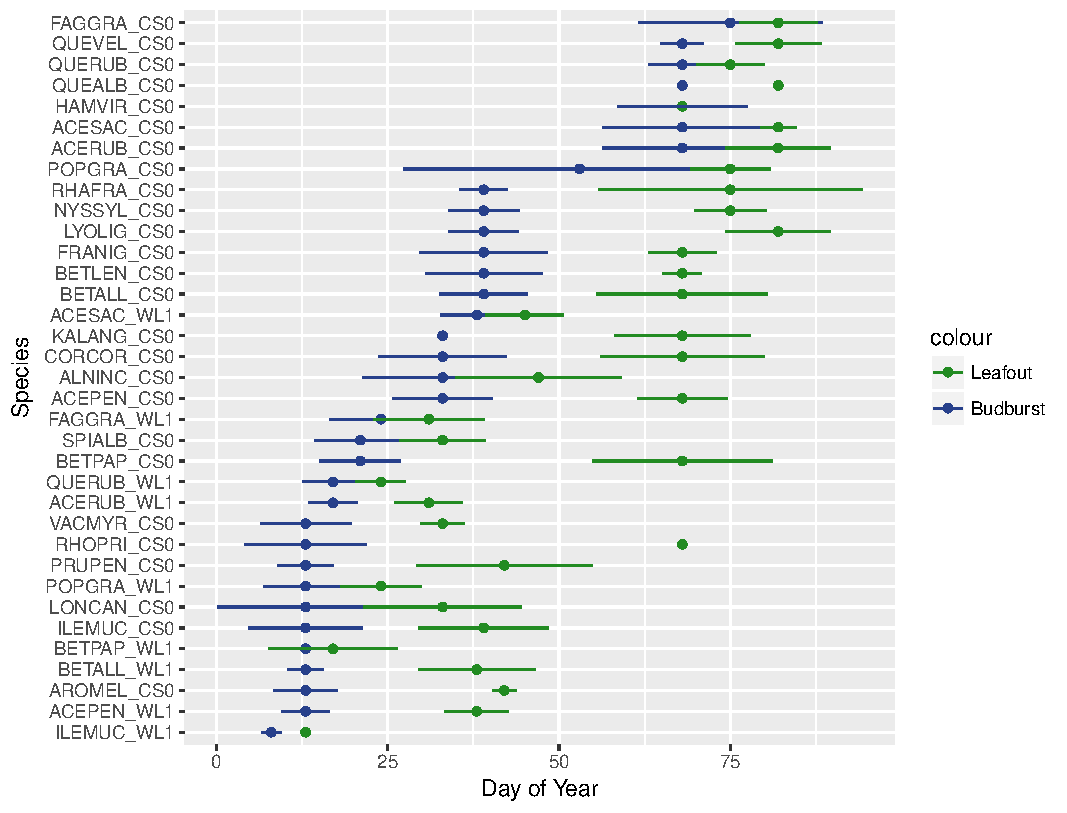
\includegraphics{..//output/Dan_TXandSp.pdf} 
\end{center}
\end{figure}

% latex table generated in R 3.2.2 by xtable 1.8-2 package
% Mon Apr 24 13:32:04 2017
\begin{table}[ht]
\centering
\caption{Anova results for duration of vegetative risk by chilling, forcing, and photoperiod effects for each species.} 
\begin{tabular}{rrrrr}
  \hline
 & ACEPEN.Sum.Sq & ACEPEN.Df & ACEPEN.F.value & ACEPEN.Pr..F. \\ 
  \hline
chilling & 119.12 & 1.00 & 1.92 & 0.17 \\ 
  forcing & 4883.47 & 1.00 & 78.90 & 0.00 \\ 
  photoperiod & 1300.30 & 1.00 & 21.01 & 0.00 \\ 
  Residuals & 6684.85 & 108.00 &  &  \\ 
   \hline
\end{tabular}
\end{table}
% latex table generated in R 3.2.2 by xtable 1.8-2 package
% Mon Apr 24 13:32:04 2017
\begin{table}[ht]
\centering
\begin{tabular}{rrrrr}
  \hline
 & ACERUB.Sum.Sq & ACERUB.Df & ACERUB.F.value & ACERUB.Pr..F. \\ 
  \hline
chilling & 6.195E-01 & 1.000E+00 & 9.371E-03 & 9.231E-01 \\ 
  forcing & 1.742E+03 & 1.000E+00 & 2.635E+01 & 1.400E-06 \\ 
  photoperiod & 4.629E+02 & 1.000E+00 & 7.002E+00 & 9.461E-03 \\ 
  Residuals & 6.611E+03 & 1.000E+02 &  &  \\ 
   \hline
\end{tabular}
\end{table}
% latex table generated in R 3.2.2 by xtable 1.8-2 package
% Mon Apr 24 13:32:04 2017
\begin{table}[ht]
\centering
\begin{tabular}{rrrrr}
  \hline
 & ACESAC.Sum.Sq & ACESAC.Df & ACESAC.F.value & ACESAC.Pr..F. \\ 
  \hline
chilling & 1.554E+01 & 1.000E+00 & 2.174E-01 & 6.426E-01 \\ 
  forcing & 2.699E+02 & 1.000E+00 & 3.776E+00 & 5.640E-02 \\ 
  photoperiod & 2.248E+02 & 1.000E+00 & 3.145E+00 & 8.090E-02 \\ 
  Residuals & 4.575E+03 & 6.400E+01 &  &  \\ 
   \hline
\end{tabular}
\end{table}
% latex table generated in R 3.2.2 by xtable 1.8-2 package
% Mon Apr 24 13:32:04 2017
\begin{table}[ht]
\centering
\begin{tabular}{rrrrr}
  \hline
 & ALNINC.Sum.Sq & ALNINC.Df & ALNINC.F.value & ALNINC.Pr..F. \\ 
  \hline
chilling &  & 0.000E+00 &  &  \\ 
  forcing & 1.025E+03 & 1.000E+00 & 5.959E+00 & 1.929E-02 \\ 
  photoperiod & 1.985E+02 & 1.000E+00 & 1.154E+00 & 2.893E-01 \\ 
  Residuals & 6.709E+03 & 3.900E+01 &  &  \\ 
   \hline
\end{tabular}
\end{table}
% latex table generated in R 3.2.2 by xtable 1.8-2 package
% Mon Apr 24 13:32:04 2017
\begin{table}[ht]
\centering
\begin{tabular}{rrrrr}
  \hline
 & AROMEL.Sum.Sq & AROMEL.Df & AROMEL.F.value & AROMEL.Pr..F. \\ 
  \hline
chilling &  & 0.000E+00 &  &  \\ 
  forcing & 3.741E+02 & 1.000E+00 & 4.004E+01 & 1.364E-04 \\ 
  photoperiod & 1.268E+02 & 1.000E+00 & 1.357E+01 & 5.049E-03 \\ 
  Residuals & 8.408E+01 & 9.000E+00 &  &  \\ 
   \hline
\end{tabular}
\end{table}
% latex table generated in R 3.2.2 by xtable 1.8-2 package
% Mon Apr 24 13:32:04 2017
\begin{table}[ht]
\centering
\begin{tabular}{rrrrr}
  \hline
 & BETALL.Sum.Sq & BETALL.Df & BETALL.F.value & BETALL.Pr..F. \\ 
  \hline
chilling & 2.871E+02 & 1.000E+00 & 5.317E+00 & 2.267E-02 \\ 
  forcing & 1.464E+03 & 1.000E+00 & 2.711E+01 & 7.110E-07 \\ 
  photoperiod & 6.171E+02 & 1.000E+00 & 1.143E+01 & 9.506E-04 \\ 
  Residuals & 7.183E+03 & 1.330E+02 &  &  \\ 
   \hline
\end{tabular}
\end{table}
% latex table generated in R 3.2.2 by xtable 1.8-2 package
% Mon Apr 24 13:32:04 2017
\begin{table}[ht]
\centering
\begin{tabular}{rrrrr}
  \hline
 & BETLEN.Sum.Sq & BETLEN.Df & BETLEN.F.value & BETLEN.Pr..F. \\ 
  \hline
chilling &  & 0.000E+00 &  &  \\ 
  forcing & 1.383E+03 & 1.000E+00 & 1.888E+01 & 3.139E-04 \\ 
  photoperiod & 5.396E+02 & 1.000E+00 & 7.367E+00 & 1.336E-02 \\ 
  Residuals & 1.465E+03 & 2.000E+01 &  &  \\ 
   \hline
\end{tabular}
\end{table}
% latex table generated in R 3.2.2 by xtable 1.8-2 package
% Mon Apr 24 13:32:04 2017
\begin{table}[ht]
\centering
\begin{tabular}{rrrrr}
  \hline
 & BETPAP.Sum.Sq & BETPAP.Df & BETPAP.F.value & BETPAP.Pr..F. \\ 
  \hline
chilling & 4.552E+00 & 1.000E+00 & 5.543E-02 & 8.142E-01 \\ 
  forcing & 1.781E+03 & 1.000E+00 & 2.168E+01 & 7.930E-06 \\ 
  photoperiod & 1.104E+03 & 1.000E+00 & 1.345E+01 & 3.587E-04 \\ 
  Residuals & 1.051E+04 & 1.280E+02 &  &  \\ 
   \hline
\end{tabular}
\end{table}
% latex table generated in R 3.2.2 by xtable 1.8-2 package
% Mon Apr 24 13:32:04 2017
\begin{table}[ht]
\centering
\begin{tabular}{rrrrr}
  \hline
 & CORCOR.Sum.Sq & CORCOR.Df & CORCOR.F.value & CORCOR.Pr..F. \\ 
  \hline
chilling &  & 0.000E+00 &  &  \\ 
  forcing & 9.417E+02 & 1.000E+00 & 1.426E+01 & 5.059E-04 \\ 
  photoperiod & 6.602E+02 & 1.000E+00 & 9.999E+00 & 2.945E-03 \\ 
  Residuals & 2.707E+03 & 4.100E+01 &  &  \\ 
   \hline
\end{tabular}
\end{table}
% latex table generated in R 3.2.2 by xtable 1.8-2 package
% Mon Apr 24 13:32:04 2017
\begin{table}[ht]
\centering
\begin{tabular}{rrrrr}
  \hline
 & FAGGRA.Sum.Sq & FAGGRA.Df & FAGGRA.F.value & FAGGRA.Pr..F. \\ 
  \hline
chilling & 6.029E+01 & 1.000E+00 & 1.365E+00 & 2.468E-01 \\ 
  forcing & 7.223E+02 & 1.000E+00 & 1.636E+01 & 1.396E-04 \\ 
  photoperiod & 2.083E+00 & 1.000E+00 & 4.718E-02 & 8.287E-01 \\ 
  Residuals & 2.914E+03 & 6.600E+01 &  &  \\ 
   \hline
\end{tabular}
\end{table}
% latex table generated in R 3.2.2 by xtable 1.8-2 package
% Mon Apr 24 13:32:04 2017
\begin{table}[ht]
\centering
\begin{tabular}{rrrrr}
  \hline
 & FRANIG.Sum.Sq & FRANIG.Df & FRANIG.F.value & FRANIG.Pr..F. \\ 
  \hline
chilling &  & 0.000E+00 &  &  \\ 
  forcing & 1.094E+03 & 1.000E+00 & 2.311E+01 & 2.420E-05 \\ 
  photoperiod & 5.191E+02 & 1.000E+00 & 1.096E+01 & 2.043E-03 \\ 
  Residuals & 1.799E+03 & 3.800E+01 &  &  \\ 
   \hline
\end{tabular}
\end{table}
% latex table generated in R 3.2.2 by xtable 1.8-2 package
% Mon Apr 24 13:32:04 2017
\begin{table}[ht]
\centering
\begin{tabular}{rrrrr}
  \hline
 & HAMVIR.Sum.Sq & HAMVIR.Df & HAMVIR.F.value & HAMVIR.Pr..F. \\ 
  \hline
chilling &  & 0.000E+00 &  &  \\ 
  forcing & 9.204E+01 & 1.000E+00 & 3.368E+00 & 8.067E-02 \\ 
  photoperiod & 5.042E+00 & 1.000E+00 & 1.845E-01 & 6.719E-01 \\ 
  Residuals & 5.739E+02 & 2.100E+01 &  &  \\ 
   \hline
\end{tabular}
\end{table}
% latex table generated in R 3.2.2 by xtable 1.8-2 package
% Mon Apr 24 13:32:04 2017
\begin{table}[ht]
\centering
\begin{tabular}{rrrrr}
  \hline
 & ILEMUC.Sum.Sq & ILEMUC.Df & ILEMUC.F.value & ILEMUC.Pr..F. \\ 
  \hline
chilling & 2.563E+01 & 1.000E+00 & 1.045E+00 & 3.084E-01 \\ 
  forcing & 2.263E+03 & 1.000E+00 & 9.228E+01 & 5.390E-17 \\ 
  photoperiod & 1.036E+03 & 1.000E+00 & 4.226E+01 & 1.400E-09 \\ 
  Residuals & 3.335E+03 & 1.360E+02 &  &  \\ 
   \hline
\end{tabular}
\end{table}
% latex table generated in R 3.2.2 by xtable 1.8-2 package
% Mon Apr 24 13:32:04 2017
\begin{table}[ht]
\centering
\begin{tabular}{rrrrr}
  \hline
 & KALANG.Sum.Sq & KALANG.Df & KALANG.F.value & KALANG.Pr..F. \\ 
  \hline
chilling &  & 0.000E+00 &  &  \\ 
  forcing & 1.362E+03 & 1.000E+00 & 1.022E+01 & 1.513E-02 \\ 
  photoperiod & 1.146E+03 & 1.000E+00 & 8.597E+00 & 2.196E-02 \\ 
  Residuals & 9.330E+02 & 7.000E+00 &  &  \\ 
   \hline
\end{tabular}
\end{table}
% latex table generated in R 3.2.2 by xtable 1.8-2 package
% Mon Apr 24 13:32:04 2017
\begin{table}[ht]
\centering
\begin{tabular}{rrrrr}
  \hline
 & LONCAN.Sum.Sq & LONCAN.Df & LONCAN.F.value & LONCAN.Pr..F. \\ 
  \hline
chilling &  & 0.000E+00 &  &  \\ 
  forcing & 2.647E+02 & 1.000E+00 & 9.722E+00 & 3.834E-03 \\ 
  photoperiod & 5.067E+02 & 1.000E+00 & 1.861E+01 & 1.440E-04 \\ 
  Residuals & 8.714E+02 & 3.200E+01 &  &  \\ 
   \hline
\end{tabular}
\end{table}
% latex table generated in R 3.2.2 by xtable 1.8-2 package
% Mon Apr 24 13:32:04 2017
\begin{table}[ht]
\centering
\begin{tabular}{rrrrr}
  \hline
 & LYOLIG.Sum.Sq & LYOLIG.Df & LYOLIG.F.value & LYOLIG.Pr..F. \\ 
  \hline
chilling &  & 0.000E+00 &  &  \\ 
  forcing & 2.028E+03 & 1.000E+00 & 4.470E+01 & 2.160E-06 \\ 
  photoperiod & 7.641E+01 & 1.000E+00 & 1.684E+00 & 2.099E-01 \\ 
  Residuals & 8.621E+02 & 1.900E+01 &  &  \\ 
   \hline
\end{tabular}
\end{table}
% latex table generated in R 3.2.2 by xtable 1.8-2 package
% Mon Apr 24 13:32:04 2017
\begin{table}[ht]
\centering
\begin{tabular}{rrrrr}
  \hline
 & NYSSYL.Sum.Sq & NYSSYL.Df & NYSSYL.F.value & NYSSYL.Pr..F. \\ 
  \hline
chilling &  & 0.000E+00 &  &  \\ 
  forcing & 1.270E+03 & 1.000E+00 & 3.136E+01 & 1.760E-05 \\ 
  photoperiod & 3.174E+02 & 1.000E+00 & 7.839E+00 & 1.106E-02 \\ 
  Residuals & 8.098E+02 & 2.000E+01 &  &  \\ 
   \hline
\end{tabular}
\end{table}
% latex table generated in R 3.2.2 by xtable 1.8-2 package
% Mon Apr 24 13:32:04 2017
\begin{table}[ht]
\centering
\begin{tabular}{rrrrr}
  \hline
 & POPGRA.Sum.Sq & POPGRA.Df & POPGRA.F.value & POPGRA.Pr..F. \\ 
  \hline
chilling & 3.771E+01 & 1.000E+00 & 5.452E-01 & 4.621E-01 \\ 
  forcing & 2.412E+03 & 1.000E+00 & 3.488E+01 & 5.070E-08 \\ 
  photoperiod & 1.013E+03 & 1.000E+00 & 1.465E+01 & 2.282E-04 \\ 
  Residuals & 6.778E+03 & 9.800E+01 &  &  \\ 
   \hline
\end{tabular}
\end{table}
% latex table generated in R 3.2.2 by xtable 1.8-2 package
% Mon Apr 24 13:32:04 2017
\begin{table}[ht]
\centering
\begin{tabular}{rrrrr}
  \hline
 & PRUPEN.Sum.Sq & PRUPEN.Df & PRUPEN.F.value & PRUPEN.Pr..F. \\ 
  \hline
chilling &  & 0.000E+00 &  &  \\ 
  forcing & 1.977E+03 & 1.000E+00 & 2.522E+01 & 8.970E-06 \\ 
  photoperiod & 4.028E+02 & 1.000E+00 & 5.139E+00 & 2.836E-02 \\ 
  Residuals & 3.449E+03 & 4.400E+01 &  &  \\ 
   \hline
\end{tabular}
\end{table}
% latex table generated in R 3.2.2 by xtable 1.8-2 package
% Mon Apr 24 13:32:04 2017
\begin{table}[ht]
\centering
\begin{tabular}{rrrrr}
  \hline
 & QUEALB.Sum.Sq & QUEALB.Df & QUEALB.F.value & QUEALB.Pr..F. \\ 
  \hline
chilling &  & 0.000E+00 &  &  \\ 
  forcing & 3.101E+02 & 1.000E+00 & 1.810E+00 & 2.154E-01 \\ 
  photoperiod & 5.637E+01 & 1.000E+00 & 3.291E-01 & 5.820E-01 \\ 
  Residuals & 1.370E+03 & 8.000E+00 &  &  \\ 
   \hline
\end{tabular}
\end{table}
% latex table generated in R 3.2.2 by xtable 1.8-2 package
% Mon Apr 24 13:32:04 2017
\begin{table}[ht]
\centering
\begin{tabular}{rrrrr}
  \hline
 & QUERUB.Sum.Sq & QUERUB.Df & QUERUB.F.value & QUERUB.Pr..F. \\ 
  \hline
chilling & 9.358E+00 & 1.000E+00 & 2.390E-01 & 6.258E-01 \\ 
  forcing & 6.977E+02 & 1.000E+00 & 1.782E+01 & 4.590E-05 \\ 
  photoperiod & 3.701E+02 & 1.000E+00 & 9.451E+00 & 2.584E-03 \\ 
  Residuals & 4.973E+03 & 1.270E+02 &  &  \\ 
   \hline
\end{tabular}
\end{table}
% latex table generated in R 3.2.2 by xtable 1.8-2 package
% Mon Apr 24 13:32:04 2017
\begin{table}[ht]
\centering
\begin{tabular}{rrrrr}
  \hline
 & QUEVEL.Sum.Sq & QUEVEL.Df & QUEVEL.F.value & QUEVEL.Pr..F. \\ 
  \hline
chilling &  & 0.000E+00 &  &  \\ 
  forcing & 6.648E-01 & 1.000E+00 & 1.727E-02 & 8.971E-01 \\ 
  photoperiod & 3.051E+00 & 1.000E+00 & 7.926E-02 & 7.819E-01 \\ 
  Residuals & 6.159E+02 & 1.600E+01 &  &  \\ 
   \hline
\end{tabular}
\end{table}
% latex table generated in R 3.2.2 by xtable 1.8-2 package
% Mon Apr 24 13:32:04 2017
\begin{table}[ht]
\centering
\begin{tabular}{rrrrr}
  \hline
 & RHAFRA.Sum.Sq & RHAFRA.Df & RHAFRA.F.value & RHAFRA.Pr..F. \\ 
  \hline
chilling &  & 0.000E+00 &  &  \\ 
  forcing & 4.265E+02 & 1.000E+00 & 6.159E+00 & 2.317E-02 \\ 
  photoperiod & 1.139E+02 & 1.000E+00 & 1.645E+00 & 2.160E-01 \\ 
  Residuals & 1.247E+03 & 1.800E+01 &  &  \\ 
   \hline
\end{tabular}
\end{table}
% latex table generated in R 3.2.2 by xtable 1.8-2 package
% Mon Apr 24 13:32:04 2017
\begin{table}[ht]
\centering
\begin{tabular}{rrrrr}
  \hline
 & RHOPRI.Sum.Sq & RHOPRI.Df & RHOPRI.F.value & RHOPRI.Pr..F. \\ 
  \hline
chilling &  & 0.000E+00 &  &  \\ 
  forcing & 6.761E+02 & 1.000E+00 & 3.728E+00 & 6.856E-02 \\ 
  photoperiod & 7.172E+02 & 1.000E+00 & 3.955E+00 & 6.133E-02 \\ 
  Residuals & 3.446E+03 & 1.900E+01 &  &  \\ 
   \hline
\end{tabular}
\end{table}
% latex table generated in R 3.2.2 by xtable 1.8-2 package
% Mon Apr 24 13:32:04 2017
\begin{table}[ht]
\centering
\begin{tabular}{rrrrr}
  \hline
 & SPIALB.Sum.Sq & SPIALB.Df & SPIALB.F.value & SPIALB.Pr..F. \\ 
  \hline
chilling &  & 0.000E+00 &  &  \\ 
  forcing & 5.414E+01 & 1.000E+00 & 1.223E+00 & 2.783E-01 \\ 
  photoperiod & 2.387E+01 & 1.000E+00 & 5.390E-01 & 4.690E-01 \\ 
  Residuals & 1.240E+03 & 2.800E+01 &  &  \\ 
   \hline
\end{tabular}
\end{table}
% latex table generated in R 3.2.2 by xtable 1.8-2 package
% Mon Apr 24 13:32:04 2017
\begin{table}[ht]
\centering
\begin{tabular}{rrrrr}
  \hline
 & VACMYR.Sum.Sq & VACMYR.Df & VACMYR.F.value & VACMYR.Pr..F. \\ 
  \hline
chilling &  & 0.000E+00 &  &  \\ 
  forcing & 5.498E+02 & 1.000E+00 & 1.560E+01 & 2.936E-04 \\ 
  photoperiod & 6.238E+01 & 1.000E+00 & 1.769E+00 & 1.906E-01 \\ 
  Residuals & 1.481E+03 & 4.200E+01 &  &  \\ 
   \hline
\end{tabular}
\end{table}



\end{document}
